%
% 第二章
%
\chapter{相关技术介绍}

%
% 2.1节
%
\section{UEFI概述}
本章将会介绍UEFI系统中关系到本文关键技术的基础内容,其中具体包括了UEFI基本结构、UEFI固件存储格式、
UEFI文件系统协议栈相关内容及驱动程序介绍,还包括基板管理控制器BMC及可信计算的基础内容。

\subsection{UEFI系统结构}
UEFI(Unified Extensible Firmware Interface,统一可扩展固件接口)定义了操作系统和平台固件直接的接口,
UEFI 提供了一个统一可扩展的固件平台,并针对平台特性定义了一系列接口。该平台整体处于硬件与操作系统中间,
平台最上层的可扩展固件接口包含了平台提供的 API 函数、启动时服务(EFI  Boot  Services)、运行时服务
(EFI  Runtime Services)和操作系统引导程序\cite{english21},下层则是根据 UEFI 规范实现的平台固件。
UEFI的平台架构
如图 2-1 所示:

\begin{figure}[htb]
    %\label{infrastructure_of_uefi}
    % 调整图片与上文的垂直距离 %
    \vspace{0cm}
    % 调整图片图片与中文标题、中文标题与英文标题距离 % 
    \setlength{\abovecaptionskip}{0.3cm}
    % 引用/fig/目录中的图片文件 %
	\centering
    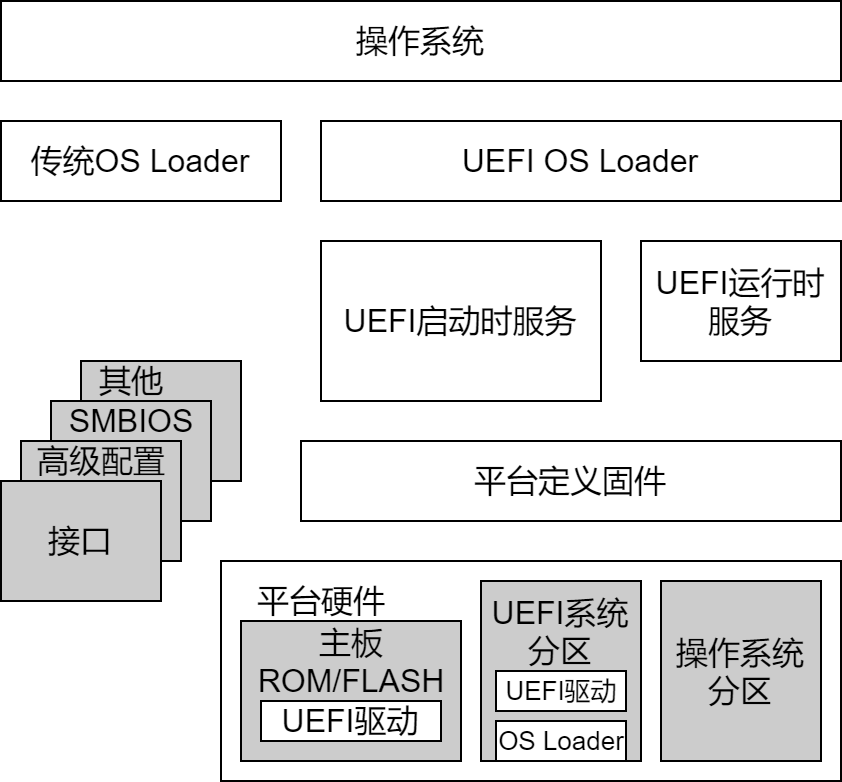
\includegraphics[width=8cm]{infrastructure_of_uefi2.png}
    % 中文标题 %
    \caption*{图 2-1 UEFI系统框架图}
    % 调整图片英文标题与下文距离 %
    \setlength{\belowcaptionskip}{-0.7cm}
    % 英文标题 %
    \caption*{Fig.2-1 Infrastructure of UEFI}
\end{figure}

\par 图 2-1 描绘了UEFI框架中各模块的关系,UEFI固件作为承上启下的模块,对底层硬件进行了抽象处理,
又不断地对上层的操作系统提供服务,并在不同的服务层的连接中采用了标准的接口。图中UEFI保留了对
传统BIOS引导操作系统的兼容性,所以在可扩展固件接口的实现中有两种操作系统引导方式,分别为
Legacy OS Loader 和UEFI OS Loader。 
\par UEFI允许操作系统预处理,实现了操作系统的引导和一些系统软件执行所需要的其它应用程序,
如诊断程序、UEFI Shell、系统调试软件等,这些程序统称为UEFI实体(UEFI Image)。根据UEFI规范,
UEFI Image包含三种:UEFI应用程序、UEFI驱动和OS Loaders,这些实体都是在UEFI API调用的基础上
实现的。
\par 从图中可以看出,UEFI的启动时服务Boot Service中包含了UEFI在PEI和DXE两个主要加载驱动完成
系统初始化过程中所需要的驱动程序、内存管理、设备管理、协议贮存等信息。而UEFI的启动时服务也有他
自己的生命周期,从下图就可以看出启动时服务在UEFI启动过程中的位置。

\begin{figure}[htb]
    %\label{bootint_sequence}
    % 调整图片与上文的垂直距离 %
    \vspace{0cm}   
    % 调整图片图片与中文标题、中文标题与英文标题距离 %                             
    \setlength{\abovecaptionskip}{0.3cm}  
    % 引用/fig/目录中的图片文件 %
	\centering
    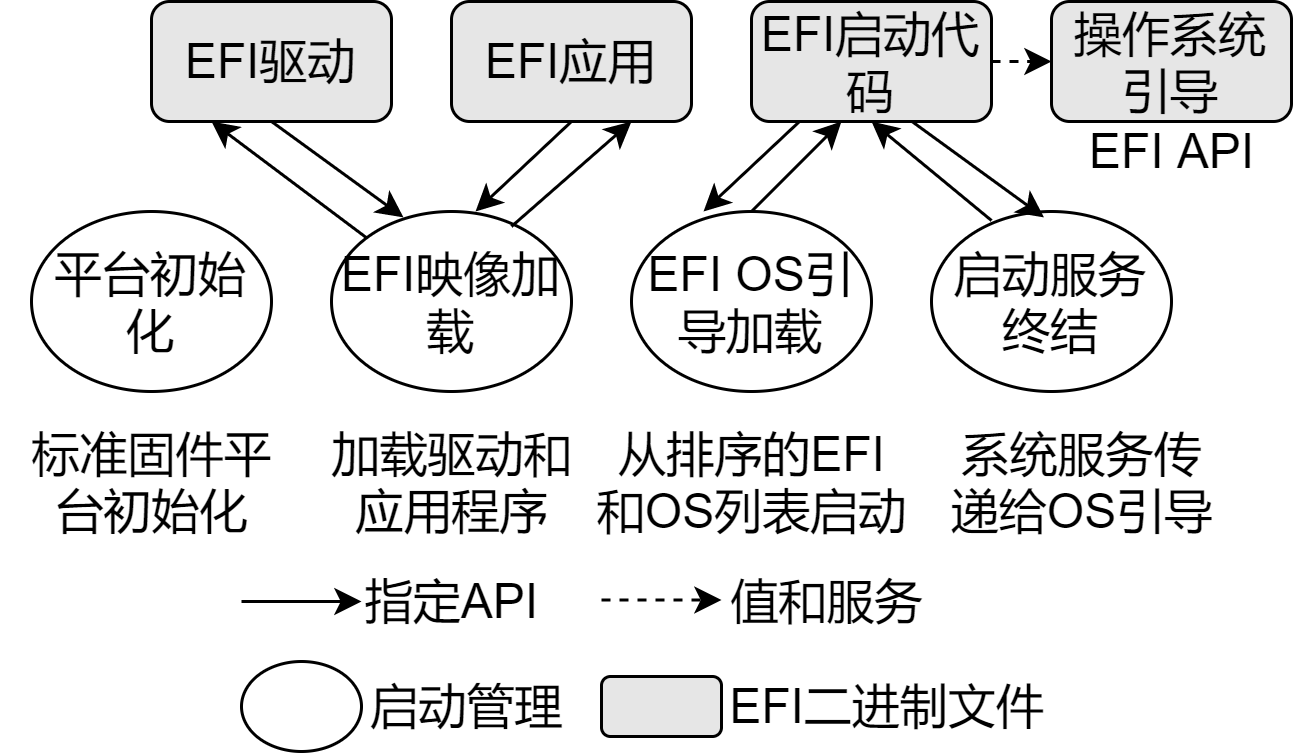
\includegraphics[width=8cm]{boot_seq2.png}
    % 中文标题 %
    \caption*{图 2-2 统一可扩展固件接口启动流程图}
    % 调整图片英文标题与下文距离 %
    \setlength{\belowcaptionskip}{-0.7cm}
    % 英文标题 %
    \caption*{Fig.2-2 Booting Sequence of UEFI}
\end{figure}

从图2-2中可以看出,Platform Init平台初始化过程中建立Boot Service系统服务和RunTime Service系统服务,
EFI Image Load阶段包括了
PEI和DXE两个主要驱动加载过程,负责加载BIOS固件中的UEFI驱动和UEFI应用程序的EFI可执行文件,之后在启动
设备选择也就是BDS阶段中,通过用户的选择,UEFI BIOS选择适当的操作系统引导程序进行加载,并同时退出
Boot Service服务,并继续向上层操作系统提供RunTime Service服务。因而在操作系统运行过程中,可以继续使
用底层UEFI BIOS提
供的运行时服务。结合图2-1也可以发现,UEFI的一些关键驱动程序,和OS Loader也会存放在如硬盘块设备的ESP
(EFI System Partition)系统分区中。由于本文主要对于UEFI启动过程中的DXE、BDS阶段进行安全方案设计,
因此,启动时服务其中包含的如协议加载函数等为本文的主要研究对象。

\subsection{UEFI协议运作方式}
UEFI中协议设计的思想为,由于UEFI的官方提供实现的版本为C语言实现,而C语言是一种面向过程的语言,而完全
使用面向过程的思想来管理和使用众多UEFI协议将会使程序变得非常复杂。Protocol作为一种对象来设计管理会更加
直观\cite{english13,english12}。因而UEFI中的Protocol引入了面向对象的思想,其中包括:
\begin{itemize}
\item 用struct来模拟class。
\item 用函数指针(Protocol的成员变量)模拟成员函数,此种函数的第一参数必须是指向Protocol的指针,用来
模拟this指针。
\end{itemize}
\par 从图2-1中可以看出,UEFI中的协议包含于UEFI启动时服务中(Boot Services),由启动时服务提供的功能进行
协议的加载、保存和调用等操作。其中UEFI启动时服务提供的协议相关的功能函数如表2-1所示。

\begin{table}[htb]
    %\label{tab:parametervalues}
    % 设置表内行间距 %
    \renewcommand\arraystretch{1.0}
    % 设置表题目 %
	\caption*{表 2-1 启动时服务协议功能表}
	\caption*{Tab.2-1 Boot Service Protocol Interface Functions}
    % @{\hspace{0pt}}用来表示表中每列的间隔 %
    % 以下这种方式为不带@{\extracolsep{\fill}}整行填充效果的例子
    % \begin{tabular*}{\hsize}{@{\hspace{0pt}}ccl@{\hspace{0pt}}}
    \begin{tabular*}{\hsize}{@{\hspace{20pt}}@{\extracolsep{\fill}}lcl@{\hspace{20pt}}}
    % 表上线和表头 %
	\toprule[0.75pt]
    \xiaowu 名称  &\xiaowu 类型  &\makecell[c]{\xiaowu 描述}\\
    % 表中线和表内容 %
	\midrule[0.5pt]
    \xiaowu InstallProtocolInterface   &\xiaowu Boot  &\quad \xiaowu 在设备句柄上安装一个协议接口\\
    \xiaowu UninstallProtocolInterface &\xiaowu Boot  &\quad \xiaowu 从设备句柄上移除一个协议接口\\
    \xiaowu ReinstallProtocolInterface &\xiaowu Boot  &\quad \xiaowu 在设备句柄上重新安装协议接口\\
    \xiaowu RegisterProtocolNotify     &\xiaowu Boot  &\makecell[l]{ 
                                                        \quad \xiaowu 注册一个事件,只要接口有信号为指定的\\
                                                        \xiaowu 协议安装\\
                                                        }\\
    \xiaowu LocateHandle               &\xiaowu Boot  &\quad \xiaowu 返回支持指定协议的句柄数组\\
    \xiaowu HandleProtocol             &\xiaowu Boot  &\quad \xiaowu 查询句柄以确定它是否支持指定的协议\\
    \xiaowu LocateDevicePath           &\xiaowu Boot  &\makecell[l]{
                                                        \quad \xiaowu 找到支持指定路径的设备路径上的所有设\\
                                                        \xiaowu 备协议并将句柄返回到最接近的设备路径
                                                        }\\
    \xiaowu OpenProtocol               &\xiaowu Boot  &\quad \xiaowu 将元素添加到使用协议的代理列表中接口\\
    \xiaowu CloseProtocol              &\xiaowu Boot  &\makecell[l]{
                                                        \quad \xiaowu 从代理列表中移除一个元素,也就是消耗\\
                                                        \xiaowu 一个协议接口
                                                        }\\
    \xiaowu OpenProtocolInformation    &\xiaowu Boot  &\quad \xiaowu 检索当前正在使用的代理列表协议接口\\
    \xiaowu ConnectController          &\xiaowu Boot  &\makecell[l]{
                                                        \quad \xiaowu 使用一组优先规则来找到最佳的驱动程序\\
                                                        \xiaowu 集管理一个控制器
                                                        }\\
    \xiaowu DisconnectController       &\xiaowu Boot  &\quad \xiaowu 通知一组驱动程序以停止管理控制器\\
    \xiaowu ProtocolsPerHandle         &\xiaowu Boot  &\makecell[l]{
                                                        \quad \xiaowu 检索安装在句柄上的协议列表,函数返回\\
                                                        \xiaowu 的缓冲区是自动分配的
                                                        }\\
    \xiaowu LocateHandleBuffer         &\xiaowu Boot  &\makecell[l]{
                                                        \quad \xiaowu 从句柄数据库中检索句柄列表,该列表符\\
                                                        \xiaowu 合搜索条件,返回缓冲区自动已分配
                                                        }\\
    \xiaowu LocateProtocol             &\xiaowu Boot  &\makecell[l]{
                                                        \quad \xiaowu 在句柄数据库中找到第一个支持所需协议\\
                                                        \xiaowu 的句柄\\
                                                        }\\
    \xiaowu InstallMultipleProtocolInterfaces
                                       &\xiaowu Boot  &\quad \xiaowu 将一个或多个协议接口安装到指定句柄上\\
    \xiaowu UninstallMultipleProtocolInterfaces
                                       &\xiaowu Boot  &\quad \xiaowu 从指定句柄中卸载一个或多个协议接口\\
    % 表下线 %
	\bottomrule[0.75pt]
    \end{tabular*}
    % 表格与下文距离 %
	\vspace{-0.3cm}
\end{table}

表2-1中列出了Boot Service中包含的所有UEFI协议相关的功能函数,其中最为常见的如InstallMultip
leProtocolInterfaces这样的加载协议函数,在众多UEFI应用以及底层驱动程序中都十分常见,因为他
可以同时提供出需要加载的多个协议GUID。
\par 同时,由于启动时服务提供了追踪最新安装了的新协议内容以及他们的使用情况,因此对于UEFI的启动时服务
来说,它可以安全地卸载并重新安装由UEFI驱动程序使用的协议接口。

\begin{figure}[htb]
    %\label{bootint_sequence}
    % 调整图片与上文的垂直距离 %
    \vspace{0cm}   
    % 调整图片图片与中文标题、中文标题与英文标题距离 %                             
    \setlength{\abovecaptionskip}{0.3cm}  
    % 引用/fig/目录中的图片文件 %
	\centering
    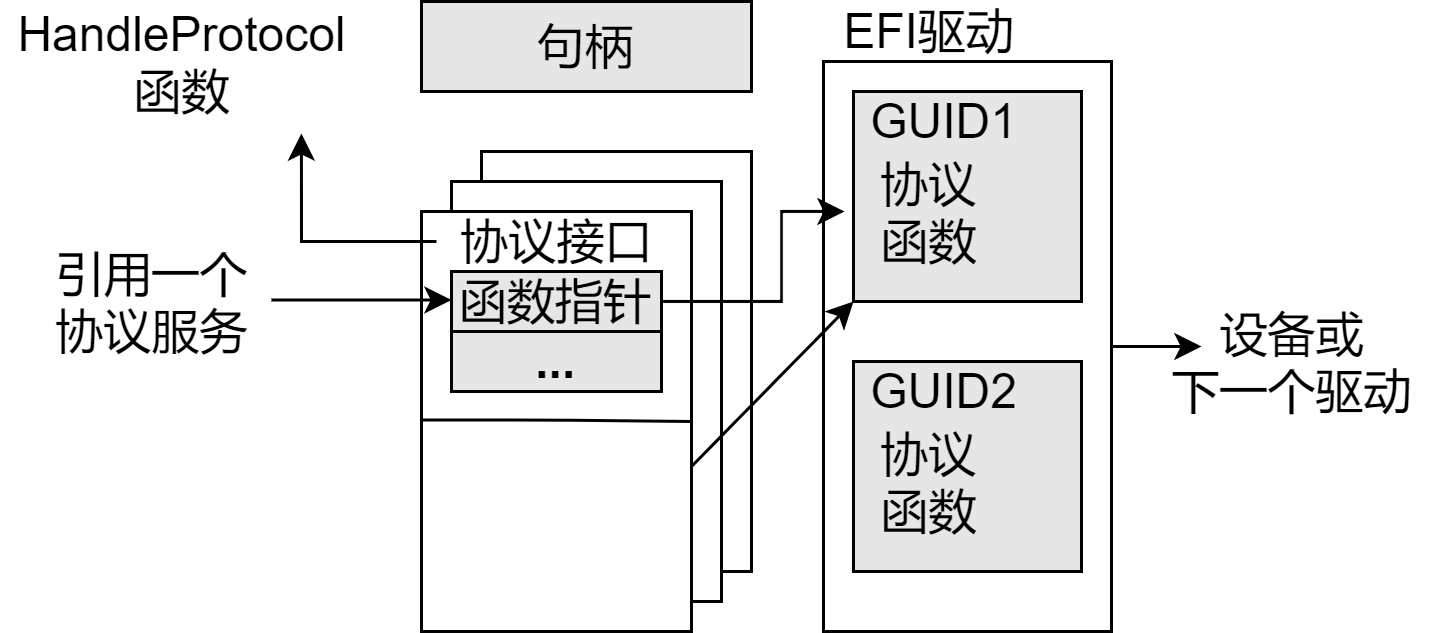
\includegraphics[width=9cm]{locate_protocol2.png}
    % 中文标题 %
    \caption*{图 2-3 统一可扩展固件接口协议加载方式图}
    % 调整图片英文标题与下文距离 %
    \setlength{\belowcaptionskip}{-0.7cm}
    % 英文标题 %
    \caption*{Fig.2-3 Locating Protocol of UEFI}
\end{figure}

\par 协议的加载过程可通过图2-3分析得知。在图2-3中可以看出,协议由HandleProtocol等表2-1中列出的装载协议
用的功能函数加载到Handle句柄上,而所有的Handle则由UEFI内核统一存储于句柄数据库,句柄数据库也是一个链表
结构用于存储记录所有的Handle句柄,这些句柄可由任意的UEFI Image(镜像)访问,从而达到函数调用的效果。而这
些协议中包含的是指向具体函数的C语言中的函数指针,这些具体函数则是在DXE阶段由UEFI系统表提供的加载驱动镜像函数
加载并驻留在内存中的。

%
% 2.2节
%
\section{UEFI固件文件系统数据存储方式介绍}
UEFI固件文件系统指的是BIOS闪存芯片中的数据存储格式,它通过统一的固件文件系统标准用来统一闪存芯片中的文件
内容和UEFI启动阶段内存中文件的内容\cite{chinese21}。具体的固件中UEFI可执行程序文件存储格式如图2-4所示。

\begin{figure}[htb]
    %\label{ffs_format}
    % 调整图片与上文的垂直距离 %
    \vspace{0cm}   
    % 调整图片图片与中文标题、中文标题与英文标题距离 %                             
    \setlength{\abovecaptionskip}{0.3cm}  
    % 引用/fig/目录中的图片文件 %
	\centering
    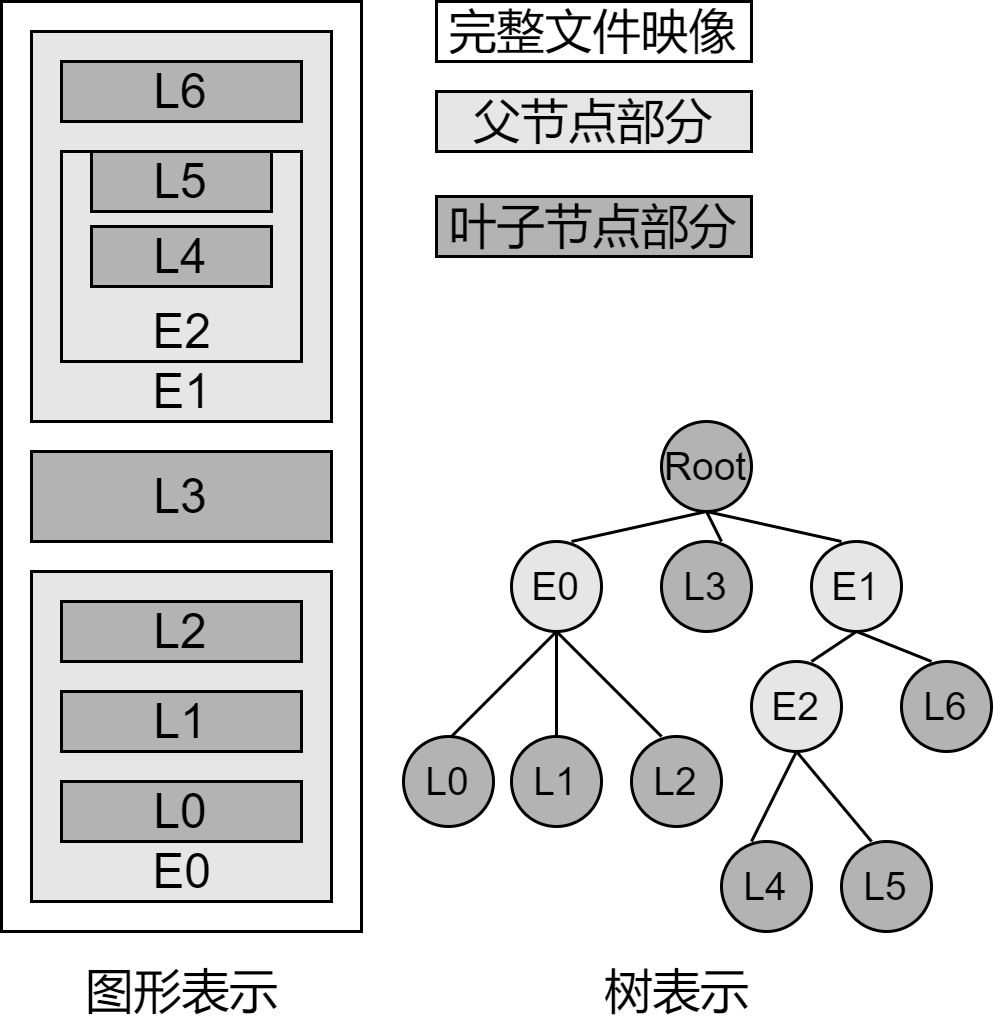
\includegraphics[width=7cm]{ffs_struct2.png}
    % 中文标题 %
    \caption*{图 2-4 固件文件系统文件存储格式}
    % 调整图片英文标题与下文距离 %
    \setlength{\belowcaptionskip}{-0.4cm}
    % 英文标题 %
    \caption*{Fig.2-4 Firmware file system file storage format}
\end{figure}

在图2-4中,左边为通过结构图的方式说明固件文件系统的数据存储格式,右边为通过数据结构中的树形结构来阐述
FFS中的文件存储。右图中,白色方框代表了一个完整的FFS中的文件映像也就是UEFI中可执行文件的二进制数据,
灰色方框代表了一个父目录结构,灰色方框中包含的深灰色方框代表了父目录中的子目录,也就是文件影响中的最小
单位。对应到右图的树结构中,灰色节点就是树中有子节点的父节点,而深灰色节点则代表了叶子节点。了解固件文件
系统中的文件数据存储格式有助于理解UEFI内核在系统初始化过程中调用相关解析FFS中文件函数的运行过程,也有
助于帮助分析本文安全方案中可信度量的具体数据内容。
%
% 2.3节
%
\section{UEFI文件系统协议栈}
UEFI BIOS中的文件系统协议栈指的是针对块设备,也就是对应一般应用于PC和服务器上的硬盘设备,UEFI文件
系统协议栈通过把对硬盘设备的不同操作功能分层起到区分和满足应用层与内核层不同功能需要的目的,下面本
节将做具体的介绍。
\subsection{总体介绍}
UEFI BIOS和传统BIOS都支持硬盘的读写功能。UEFI优于传统BIOS的地方在于,UEFI还提供了对文件系统的支持
\cite{english18}。
其中传统BIOS由于直接由汇编语言编写,实现内容十分依赖于具体的硬件平台,因此不易在运行流程中进行像对硬盘
设备这种次要设备的过多交互,像ESP(EFI System Partition)分区中文件的操作也就只通过直接操作硬盘驱动
程序来存取具体扇区中的数据内容。然而进入了UEFI时代,BIOS的实现得到了以C语言为具体实现工具并进行了国际
统一的实现标准,提供统一固件接口,因此从需求性和实现性方面都更加需要UEFI系统与硬盘的交互功能,因此才
出现了用于管理UEFI中硬盘设备文件的UEFI文件系统协议栈。
\par 通常,每个UEFI系统至少有一个ESP分区,在这个分区上存放了操作系统启动文件。既然操作系统加载器以
文件的形式存放在ESP分区内,UEFI就需要有读写文件的功能。文件的读写与管理在一定需求量和为了统一便捷的前
提下必须通过文件系统来完成,要支持读写文件,UEFI必须首先能操作ESP分区上的文件系统。ESP主要用来存放
操作系统加载器相关的文件,有时在一些实际项目的调试过程中,也需要通过将事先编译好的EFI可运行特定硬件的
驱动程序通过操作系统放入UEFI能访问到的ESP分区内,并从UEFI SHELL中手动加载所述驱动程序来使调试工作
更加便捷。总体来说,UEFI对文件系统的要求比较简单,所以采用FAT文件系统就可以满足需求,随着UEFI技术的
不断发展,对硬盘数据访问的要求也越来越高,因此目前已出现ext2等文件系统用来支持UEFI,并已发布到官方
开源库中。UEFI文件系统协议栈图如图2-5所示。

\begin{figure}[htb]
    %\label{ffs_format}
    % 调整图片与上文的垂直距离 %
    \vspace{0cm}   
    % 调整图片图片与中文标题、中文标题与英文标题距离 %                             
    \setlength{\abovecaptionskip}{0.3cm}  
    % 引用/fig/目录中的图片文件 %
	\centering
    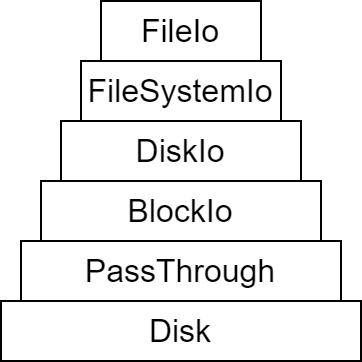
\includegraphics[width=4cm]{filesystem_protocol_stack2.png}
    % 中文标题 %
    \caption*{图 2-5 统一可扩展固件接口文件系统协议栈}
    % 调整图片英文标题与下文距离 %
    \setlength{\belowcaptionskip}{-0.7cm}
    % 英文标题 %
    \caption*{Fig.2-5 UEFI File system protocol stack}
\end{figure}

如图2-5所示,最下层Disk层表示如硬盘设备这样的块设备硬件。PassTh-\newline rough层表示硬盘设备与总线接口的协议,
EFI\_ATA\_PASS\_THRU\_PROTOCOL提供有关ATA控制器以及将ATA命令块发送到与该ATA控制器相连的任何ATA设备的信息。
而EXT\_SCSI\_PASS\_THRU\_PROTOCOL协议提供了将ATAPI命令块发送到连接到该ATA控制器或SCSI控制器的ATAPI设备
的功能。此协议可直接操作硬盘具体扇区中的数据内容,为UEFI内核提供最底层的硬盘接口功能函数。
\par 再往上一层是块输入输出BlockIo(下同)层,BlockIo是可扩展固件接口输入输出协议EFI\_BLOCK\_IO\_PROTOCOL
的缩写,主要提供了按块访问设备的功能,包括块的读写函数和刷新flush函数。再往上一层的硬盘输入输出DiskIo层,
在BlockIo的基础上进行再次封装,DiskIo为EFI\_DISK\_IO\_PROTOCOL的缩写。此协议提供了从磁盘任
意地址读写任意长度数据的功能,这也符合了硬盘作为块设备可以随机访问数据的特点。
\par 再往上一层为文件系统输入输出FileSystemIo(下同)层,他对应于简易文件系统协议EFI\_SIMPLE\_FILE\_SYSTEM
\_PROTOCOL协议,这个协议是对文件系统驱动加载时,驻留在内存中的文件系统功能函数的引用和封装。再往上一层为文件
输入输出FileIo层,对应于EFI\_FILE\_PROTOCOL协议,用于对以文件为单位的数据进行操作。在UEFI运行环境中如Shell环
境中加载.efi文件时,就经历了从下到上完整的协议栈的过程,最终以文件数据流的形式传递给Shell环境,并完成后续的执
行或其他加载操作。

\subsection{相关驱动介绍}
UEFI中的驱动大致分为两类:一类是符合UEFI驱动模型的驱动,成为“UEFI驱动”;另一类是不遵循UEFI驱动模型的驱动,
称为“DXE驱动”,也称为服务型驱动。服务型驱动加载过程较为简单,在Image初始化的时候,即在执行模块入口函数时,
将Protocol安装到自身Handle即可。
如2.1节中UEFI协议运作方式的介绍可知,UEFI协议作为一个包含了所需功能函数指针的结构体,需要具体的UEFI驱动程序
为其实现所需的功能。
UEFI文件系统协议栈相关的驱动程序分别为:AtaatapiPassThruDxe、PartitionDxe、DiskIoDxe、FileSysDxe,
从命名可以看出,他们四个驱动都属于DXE驱动即服务型驱动,用于在UEFI的DXE和BDS阶段为系统提供服务,其中
的PassThruDxe和FileSysDxe根据具体的硬盘接口与具体文件系统不同而定。其中PassThruDxe驱动程序负责定义硬盘设备
与ATA或SCSI总线进行数据交互的功能;PartitionDxe用于解析存储在硬盘ESP分区中的GPT分区表,用于获取到硬盘中数据
的分区信息,磁盘在使用前都要进行分区,也就是将硬盘划分为一个个逻辑的区域,不同的分区上可装载不同的文件系统,以
方便用户使用。
GPT分区表(GUID Partition Table):全局唯一标识磁盘分区表\cite{extra3},是一个实体硬盘的
分区表的结构布局的标准,是可扩展固件接口(EFI)标准,被用于替代BIOS系统中的一64bits来存储逻辑块地址和大小信
息的主开机纪录(MBR)分区表,与普遍使用的主引导记录(MBR)分区方案相比,GPT提供了更加灵活的磁盘分区机制。
LBA(Logical Block Addressing)逻辑块寻址模式将CHS这种三维寻址方式转变为一维的线性寻址,它把硬盘所有
物理扇区的C/H/S编号通过一定的规则转变为一线性的编号,系统效率得到大大提高,避免了烦琐的磁头/柱面/扇区
的寻址方式。如图中的LBA0扇区为保护MBR,它的作用是阻止不能识别GPT分区的磁盘工具试图对其进行分区或格式化
等操作。LBA1扇区开始则为分区表和表项,每个表项对应一个用户区域内的磁盘分区,并表识这个分区的开始和结束
位置。关于GPT分区表的详细分析及恶意篡改方式将在第三章中介绍。

%\begin{figure}[htb]
    %\label{ffs_format}
    % 调整图片与上文的垂直距离 %
    %\vspace{0cm}   
    % 调整图片图片与中文标题、中文标题与英文标题距离 %
    %\setlength{\abovecaptionskip}{0.3cm}  
    % 引用/fig/目录中的图片文件 %
	%\centering
    %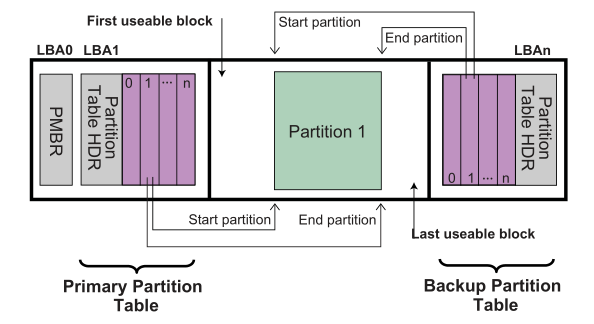
\includegraphics[width=10cm]{partition.png}
    % 中文标题 %
    %\caption*{图 2-6 硬盘全局分区表示意图}
    % 调整图片英文标题与下文距离(本文标准为-0.7cm) %
    %\setlength{\belowcaptionskip}{-0.7cm}
    % 英文标题 %
    %\caption*{Figure 2-6 Hard disk GPT partition}
%\end{figure}

DiskIoDxe驱动用于定义硬盘最基础的输入输出数据功能,也就是等同于操作系统中的硬盘驱动程序;而
FileSysDxe驱动则负责为UEFI提供与硬盘硬件相同的文件系统数据组织形式,用以在UEFI系统中通过UNIX风格的文件系统
为其他模块提供硬盘文件的交互功能支持。
%
% 2.4节
%
\section{BMC技术介绍}
BMC(Baseboard Management Controller)基板管理控制器是一种用于实时检测服务器硬件信息并具备独立运算能力的
计算机系统中的组件,它通过IPMI协议与服务器中的其他硬件设备进行通信。在基于IPMI协议的管理平
台中,系统对平台各个硬件设备的信息管理策略,都是通过与BMC通信并统计运算而实现
的\cite{addition5,addition6}。BMC拥有除了独立处理器外的独立固件闪存、系统电源、网卡设备,是一个具有独立性的基于服务器平台的管理
子系统。在如今的服务器国产化过程中,BMC越来越得到各个厂商的广泛使用。

\subsection{BMC与BIOS通讯方式}
IPMI协议作为BMC与服务器其他硬件设备通信的桥梁主要有两种通信方式,他们分别是BT(Block Transfer)接口
和KCS(Keyboard Controller Style)接口,其中BT接口主要是用于传输数据的块传输,即最小传输单位设置为一块,
256字节。而KCS接口主要用于以最小单位为一字节来进行数据传输。而在BIOS与BMC的通信过程中,主要使用BMC来
进行一些度量过程中基准值的存储功能,因此使用KCS接口来进行通讯设计,以避免不必要的传输资源浪费。

\begin{figure}[htb]
    %\label{ffs_format}
    % 调整图片与上文的垂直距离 %
    \vspace{0cm}   
    % 调整图片图片与中文标题、中文标题与英文标题距离 %
    \setlength{\abovecaptionskip}{0.3cm}  
    % 引用/fig/目录中的图片文件 %
	\centering
    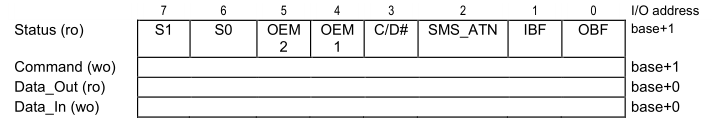
\includegraphics[width=14cm]{kcs_register.png}
    % 中文标题 %
    \caption*{图 2-6 KCS接口寄存器信息}
    % 调整图片英文标题与下文距离(本文标准为-0.7cm) %
    \setlength{\belowcaptionskip}{-0.7cm}
    % 英文标题 %
    \caption*{Fig.2-6 KCS Interface Registers}
\end{figure}

如图2-7所示,为KCS接口所使用到的寄存器即相关信息,主要涉及到四个寄存器,分别是用来查看BMC此时状态的状态
寄存器、用于指定BMC命令的命令寄存器、和两个分别用来进行数据输入和数据输出缓存的寄存器。有关这些寄存器具体
使用方法和使用流程将在第四章的BMC驱动实现中做详细说明。

%
% 2.5节
%
%\section{可信计算技术}

%\subsection{可信计算信任链}

%\subsection{可信平台模块}

%
% 2.5节
%
\section{本章小结}
本章首先介绍了UEFI规范中的整体系统设计结构,并着重介绍了UEFI的协议运作方式和对本文有重要作用的启动时服务
提供的具体功能函数。然后对固件文件系统中驱动数据的存放方式进行了描述,为后面的驱动内容读取功能提供了理论基础;
分析了UEFI文件系统协议栈在系统中的作用和具体到主要的四个驱动程序名称。最后对UEFI BIOS中与BMC系统的通信方式
进行了分析,选用了IPMI的KCS访问模式,来完成数据的交互。

%\bjutclearpage